\documentclass[12pt]{Homework}

% Changed from \usepackage{prelude}
\usepackage{preamble}
\usepackage{amssymb}
\usepackage{enumitem}
\usepackage{mathrsfs}
\def\upint{\mathchoice%
    {\mkern13mu\overline{\vphantom{\intop}\mkern7mu}\mkern-20mu}%
    {\mkern7mu\overline{\vphantom{\intop}\mkern7mu}\mkern-14mu}%
    {\mkern7mu\overline{\vphantom{\intop}\mkern7mu}\mkern-14mu}%
    {\mkern7mu\overline{\vphantom{\intop}\mkern7mu}\mkern-14mu}%
  \int}
\def\lowint{\mkern3mu\underline{\vphantom{\intop}\mkern7mu}\mkern-10mu\int}
\usepackage[mathscr]{euscript}
\usepackage{comment}
\usepackage{MnSymbol}
\usepackage{tikz,float}
\usepackage{tikz-cd}
\usepackage{graphicx}
\usepackage{mathtools}
\usepackage{bbding}
\renewcommand\qedsymbol{\Peace}
\newcommand\placeqed{\nobreak\enspace\Peace}
\usepackage{caption, threeparttable}
\usepackage{halloweenmath}
\newcommand{\contradiction}{\null\hfill\large{$\mathghost$}\normalsize}
\newcommand{\im}{\mathscr{I}\text{m}}
\newcommand{\re}{\mathscr{R}\text{e}}
\newcommand{\res}{\text{Res}}

\name{Kayla Orlinsky}
\course{Complex Analysis Exam}
\term{Fall 2012}
\hwnum{Fall 2012}

\begin{document}

\begin{problem} $\,$
Evaluate the integral $$\int_0^\infty\frac{dx}{1+x^n},\qquad n\ge2$$ being careful to justify your methods. 
\end{problem}


\begin{solution}$\,$
Then we get that there is a pole at $e^{i\frac{\pi}{n}}$ which can be isolated in a pizza slice of angle $\frac{2\pi}{n}$.

Thus, we integrate around the following contour:
\begin{center}
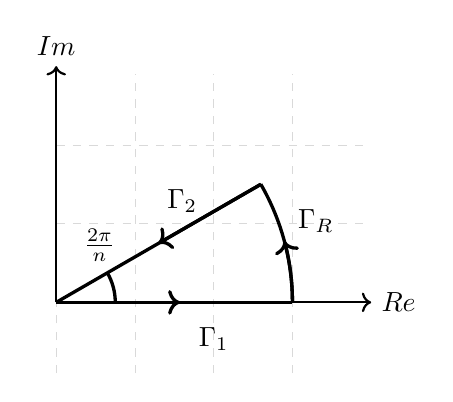
\begin{tikzpicture}
\draw[help lines, color=gray!30, dashed] (0,-0.9) grid (3.9,2.9);
\draw[->,very thick] (3,0) arc (0:15:3cm);
\draw[very thick] (3,0) arc (0:30:3cm) node[above,yshift=-0.75cm,xshift=0.7cm]{$\Gamma_R$};
\draw[->,very thick] (0,0) -- (1.57,0);
\draw[very thick] (0.75,0) -- (3,0) node[above,yshift=-0.75cm,xshift=-1cm]{$\Gamma_1$};
\draw[->,very thick] (2.6,1.5) -- (1.3,0.75);
\draw[very thick] (0,0) -- (2.6,1.5) node[above,yshift=-0.5cm,xshift=-1cm]{$\Gamma_2$};
\draw[very thick] (0.75,0) arc (0:30:0.75cm) node[above,yshift=0cm,xshift=-0.1cm]{$\frac{2\pi}{n}$};
\draw[->, thick] (0,0)--(4,0) node[right]{$Re$};
\draw[->, thick] (0,0)--(0,3) node[above]{$Im$};
\end{tikzpicture}
\end{center}

Immeidately, we get that $$|I_R|=\left|\int_{\Gamma_R}\frac{dz}{1+z^n}\right|\le\int_0^{\frac{2\pi}{n}}\frac{R}{R^n-1}d\theta=\frac{2\pi R}{n(R^n-1)}\to0\qquad R\to\infty.$$

Since $$I_2=\int_{\Gamma_2}\frac{dz}{1+z^n}=\int_R^0\frac{e^{i\frac{2\pi}{n}}dr}{1+r^ne^{2\pi i}}=-e^{i\frac{2\pi}{n}}\int_0^R\frac{dr}{1+r^n}=-e^{i\frac{2\pi}{n}}I_1.$$

Thus, using the residue theorem, we get that $$\res_{z=e^{i\frac{\pi}{n}}}\frac{1}{1+x^n}=\lim_{z\to e^{i\frac{\pi}{n}}}\frac{x-e^{i\frac{\pi}{n}}}{x^n+1}=\lim_{z\to e^{i\frac{\pi}{n}}}\frac{1}{nx^{n-1}}=\frac{1}{n}e^{-(n-1)i\frac{\pi}{n}}$$ and that $$2\pi i\frac{1}{n}e^{-(n-1)i\frac{\pi}{n}}=\lim_{R\to\infty}(I_1+I_2+I_R)=(1-e^{i\frac{2\pi}{n}})I_1$$ and so $$\int_0^\infty\frac{dx}{1+x^n}= \frac{\pi}{n}e^{-(n-1)i\frac{\pi}{n}}\frac{2i}{1-e^{i\frac{2\pi}{n}}}=\frac{\pi}{n}\frac{-2i}{e^{-i\frac{\pi}{n}}-e^{i\frac{\pi}{n}}}=\frac{\pi/n}{\sin(\pi/n)}$$
\end{solution}
\newpage

\begin{problem} $\,$
Find the Laurent series expansion for $$\frac{1}{z(z+1)}$$ valid in $\{1<|z-1|<2\}.$
\end{problem}


\begin{solution}$\,$
Since on $1<|z-1|<2$ we have that $1>\frac{1}{|z-1|}>\frac{1}{2}$ and $\frac{|z-1|}{2}<1$ so \begin{align*}
    \frac{1}{z(z+1)}&=\frac{1}{z}-\frac{1}{z+1}\\
    &=\frac{1}{(z-1)+1}-\frac{1}{(z-1)+2}\\
    &=\frac{\frac{1}{z-1}}{1+\frac{1}{z-1}}-\frac{\frac{1}{2}}{1+\frac{z-1}{2}}\\
    &=\frac{1}{z-1}\frac{1}{1-\frac{1}{1-z}}-\frac{1}{2}\frac{1}{1-\frac{1-z}{2}}\\
    &=\frac{1}{z-1}\sum_{l=0}^\infty\left(\frac{1}{1-z}\right)^l-\frac{1}{2}\sum_{k=0}^\infty\left(\frac{1-z}{2}\right)^k\\
    &=\sum_{l=0}^\infty\frac{1}{(1-z)^{l+1}}-\sum_{k=0}^\infty\frac{(1-z)^k}{2^{k+1}}
\end{align*}
\end{solution}
\newpage

\begin{problem} $\,$
Suppose that $f$ is an entire function and that there is a bounded sequence of distinct real numbers $a_1,a_2,a_3,...$ such that $f(a_k)$ is real for each $k.$ Show that $f(x)$ is real for all real $x.$
\end{problem}


\begin{solution}$\,$
It suffices to show that $f(z)$ has a Taylor Expansion with only real coefficeints. 

First, note that since $a_k$ are bounded, they have a real limit point $a$. Therefore, because $f$ is entire (namely continuous), $$\lim_{k\to\infty}f(a_k)=f\left(\lim_{k\to\infty}a_k\right)=f(a)$$ and $f(a)\in\mathbb{R}$ since $f(a_k)\in\mathbb{R}$ for all $k$.

Therefore, $$\frac{f(a_k)-f(a)}{a_k-a}\in\mathbb{R}\qquad\text{ for all }k$$ and so $f'(a)\in\mathbb{R}$.

Inductively, we get that $f^{(n)}(a)\in\mathbb{R}$ for all $n$ and so, because $f$ is entire, we can write its Taylor expansion around $a$ and get that $$f(z)=\sum_{k=0}^\infty\frac{f^{(k)}(a)}{k!}(z-a)^k$$ and since $f^{(k)}(a)/k!\in\mathbb{R}$ for all $k$ and $a\in\mathbb{R}$, we get that $f(x)\in\mathbb{R}$ for all $x\in\mathbb{R}$.
\end{solution}
\newpage





\begin{problem} $\,$
Suppose $$f_n(z)=\sum_{k=0}^n\frac{1}{k!z^k},\qquad z\not=0$$ and let $\varepsilon>0$. Show that for large enough $n,$ all the zeros of $f_n$ are in the disk $D(0,\varepsilon)$ with center $0$ and radius $\varepsilon.$
\end{problem}


\begin{solution}$\,$
First, $$\lim_{n\to\infty}f_n(z)=\sum_{k=0}^\infty\frac{\left(\frac{1}{z}\right)^k}{k!}=e^\frac{1}{z}.$$ Furthermore, this convergence is uniform. Namely, for $\varepsilon>0$, there exists $N$ such that $|f_n(z)-e^{1/z}|<\varepsilon$ for all $n\ge N$ and all $z\not=0.$

Now, if $|z|<\frac{1}{\varepsilon}$ then $$|e^z|\ge e^{-\frac{1}{\varepsilon}}$$ and so if $|z|>\varepsilon$n then $$|e^{\frac{1}{z}}|\ge e^{-\frac{1}{\varepsilon}}>0.$$

Namely, because $e^{1/z}$ has a lower bound on $|z|>\varepsilon$, so too must $f_n(z)$. Thus, the zeros of $f_n(z)$ are contained in $D(0,\varepsilon).$
\end{solution}


\end{document}
 